\chapter{Pierre Auger Observatory}\label{Ch:PAO}


Science Goals of the Pierre Auger Observatory is to probe the origins and characteristics of cosmic rays above 10$^{17}$ eV and to study the interactions of the most energetic particles observed in nature.

The Pierre Auger Observatory (PAO) is an hybrid detector that is located near Malarg\"ue in the Mendoza Province, Argentina. PAO consists of 1660 Cherenkov water detector spread over 3000 km$^2$  by 24 fluorescence telescopes. 

\begin{figure}[hp]
\centering
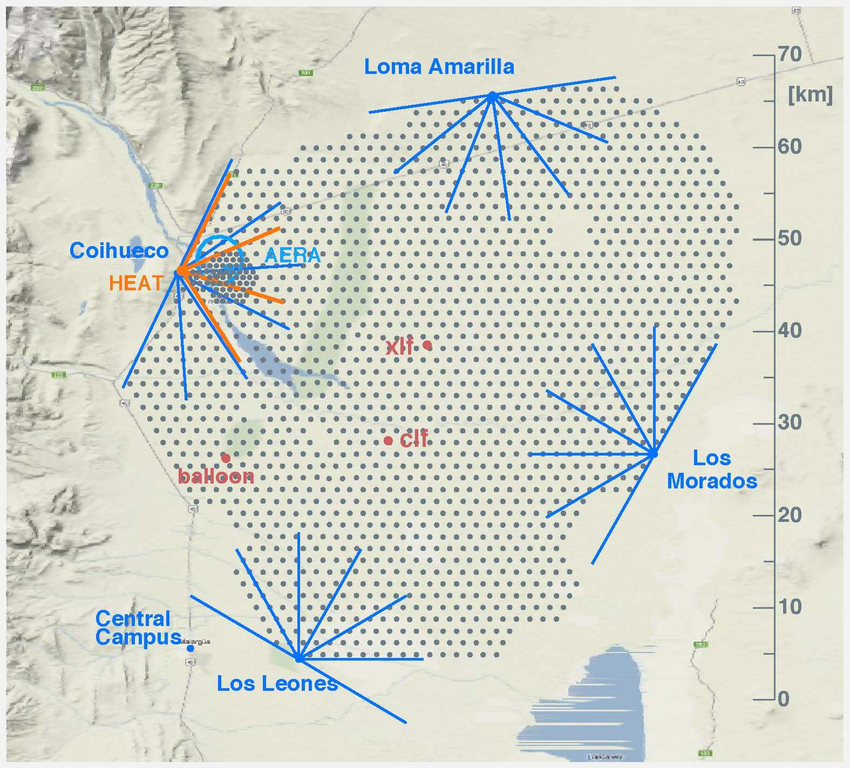
\includegraphics[width=0.7\textwidth]{chapters/pix/PAO_equipment_layout_overview.png}
\caption{Image of layout of Pierre Auger Observatory located near Malargue, Argentina.}
\label{fig:PAO_layout}
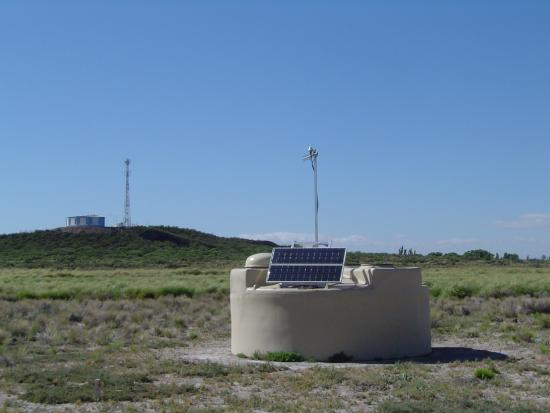
\includegraphics[width=0.7\textwidth]{chapters/pix/pierre-auger-observatory_tankAndTelescope.jpg}
\caption{Image of one of the fluorescence detector site (background) and one of the surface detectors (foreground).}
\label{fig:PAO_TankAndTelescope}
\end{figure}


\section{Surface Detector}

\begin{figure}
\centering
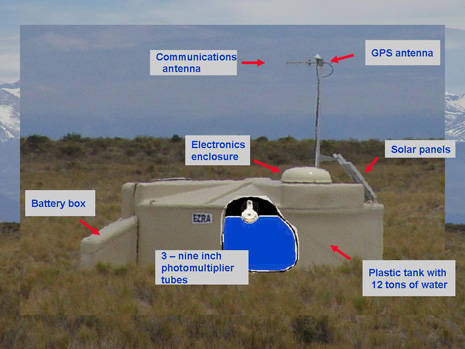
\includegraphics[width=0.7\textwidth]{chapters/pix/inside_surface_detector.jpg}
\caption{Basic schematic of a surface detector.}
\label{fig:SD_schematic}
\end{figure}

The surface array consists of 1660 water Cherenkov tanks. The majority of tanks are configured with a spacing of 1500 metres while there is a small subset of tanks in front of the fluorescence telescopes at the Coihueco site with spacing of 750 metres. 

The surface array has a duty cycle of nearly 100\% and the maintenance cycle is so that no more then 20 tanks are down at any one time.

\section{Fluorescence Detector}

\begin{figure}
\centering
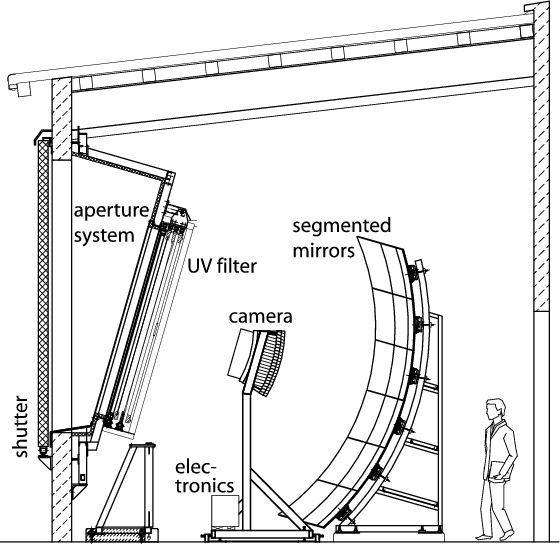
\includegraphics[width=0.7\textwidth]{chapters/pix/fluorescence_telescope.png}
\caption{Basic schematic of a fluorescence telescope.}
\label{fig:FD_schematic}
\end{figure}

There are four fluorescence detector site surrounding the surface array. At each fluorescence detector site there are six telescopes covering 180\textdegree \ in azimuth and 30\textdegree \ in elevation. At one site there are three extra telescopes with slightly greater then 90\textdegree \ in azimuth and cover 30\textdegree \ to 60\textdegree \ in elevation.

\subsection{Photomultiplier Tubes}

\section{Communication System and CDAS}

\section{Event Reconstruction}

\subsection{Surface Detector}

\subsection{Fluorescence Detector}

\section{Enhancements and future upgrades}